% \PassOptionsToPackage{table}{xcolor}
\documentclass[11pt]{beamer}
\usepackage[utf8]{inputenc}
\usepackage[english]{babel}
\usepackage{amsmath}
\usepackage{amsfonts}
\usepackage{amssymb}
\usepackage{graphicx}
\usepackage{tikz}
\usepackage{algorithm}
\usepackage{algorithmic}
\usepackage{silence,lmodern}
\usepackage{csquotes}
\usepackage[backend=bibtex, bibencoding=ascii, style=authoryear, doi=false, isbn=false,url=false, uniquename=init, giveninits=true]{biblatex}
\usepackage{multimedia}
\usepackage{dirtytalk}
\usepackage{pgfplotstable,booktabs,longtable}
\WarningFilter{biblatex}{Patching footnotes failed}

% \mode<presentation>
% {
    \usetheme[hideothersubsections]{PaloAlto}
    % \usecolortheme{beaver}
% }
\usetikzlibrary{calc,trees,positioning,arrows,chains,shapes.geometric,
decorations.pathreplacing,decorations.pathmorphing,
shapes,matrix,shapes.symbols,plotmarks,decorations.markings,
shadows,shapes.geometric,arrows}

\setbeamercolor{logo}{bg=white}  %controls the color of the logo area
\setbeamerfont{footnote}{size=\tiny}

% \addbibresource{library.bib}

\makeatletter
\setlength{\beamer@headheight}{.9cm}
\makeatother

\author{S M Al Mahi}
\title[ECEN-5283 Computer Vision]{Project 1: \\Linear Approach to Camera Calibration}
\setbeamercovered{transparent} 
\setbeamertemplate{navigation symbols}{}


\logo{
\includegraphics[width=1cm]{Oklahoma_State_University_logo.png}}
\institute{Oklahoma State University} 
\date{\today} 
\subject{}
\begin{document}

\setbeamertemplate{sidebar left}{}
\begin{frame}
\titlepage
\end{frame}

\newpage
\setbeamertemplate{sidebar left}[sidebar theme]
\section{Project Objective}
\begin{frame}
\frametitle{Project Objective}
	\begin{block}{Objectives}
	\begin{enumerate}
		\item Geometric camera calibration using linear approach
		\item Predict the 2D locations from static and moving 3D points
		\item Calculate projection matrix \textbf{M}
		\item Using M to calculate \textit{intrinsic} and \textit{extrinsic} parameters
		\item For verification visualizing the calibrated images and videos
	\end{enumerate}
	\end{block}
% \end{frame}
% \begin{frame}
	\begin{block}{Tools, Input \& Output}
	\begin{enumerate}
		\item \textbf{Python}, PyCharm IDE, Matplotlib, Numpy
		\item \textbf{Latex Beamer}, Sublime Text
		\item \textbf{Input} were \say{model.dat} and \say{obesrve.dat} files.
		\item Generated input by program.
	\end{enumerate}
	\end{block}
\end{frame}

\section{Technical Background}
\begin{frame}
\frametitle{Technical Background}
\begin{figure}
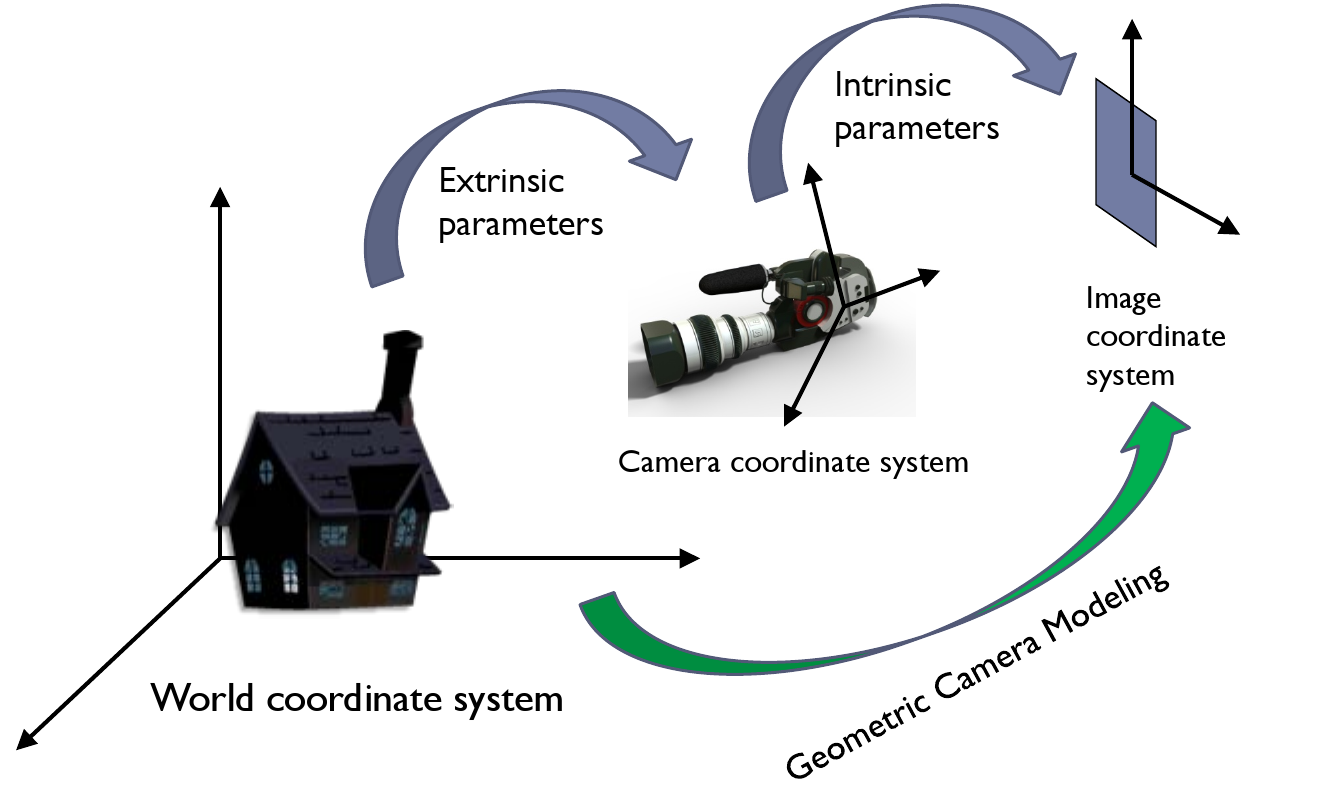
\includegraphics[width=\textwidth]{basics-1.png}
\caption{Extrinsic parameters are related to world coordinate. i.e. Rotation and Translation. Intrinsic parameters are related to camera coordinate system and hardware properties like pixel size, orientation.}
\end{figure}
\end{frame}

\subsection{Intrinsic Parameters}

\begin{frame}
\frametitle{Intrinsic Parameters}
\begin{figure}
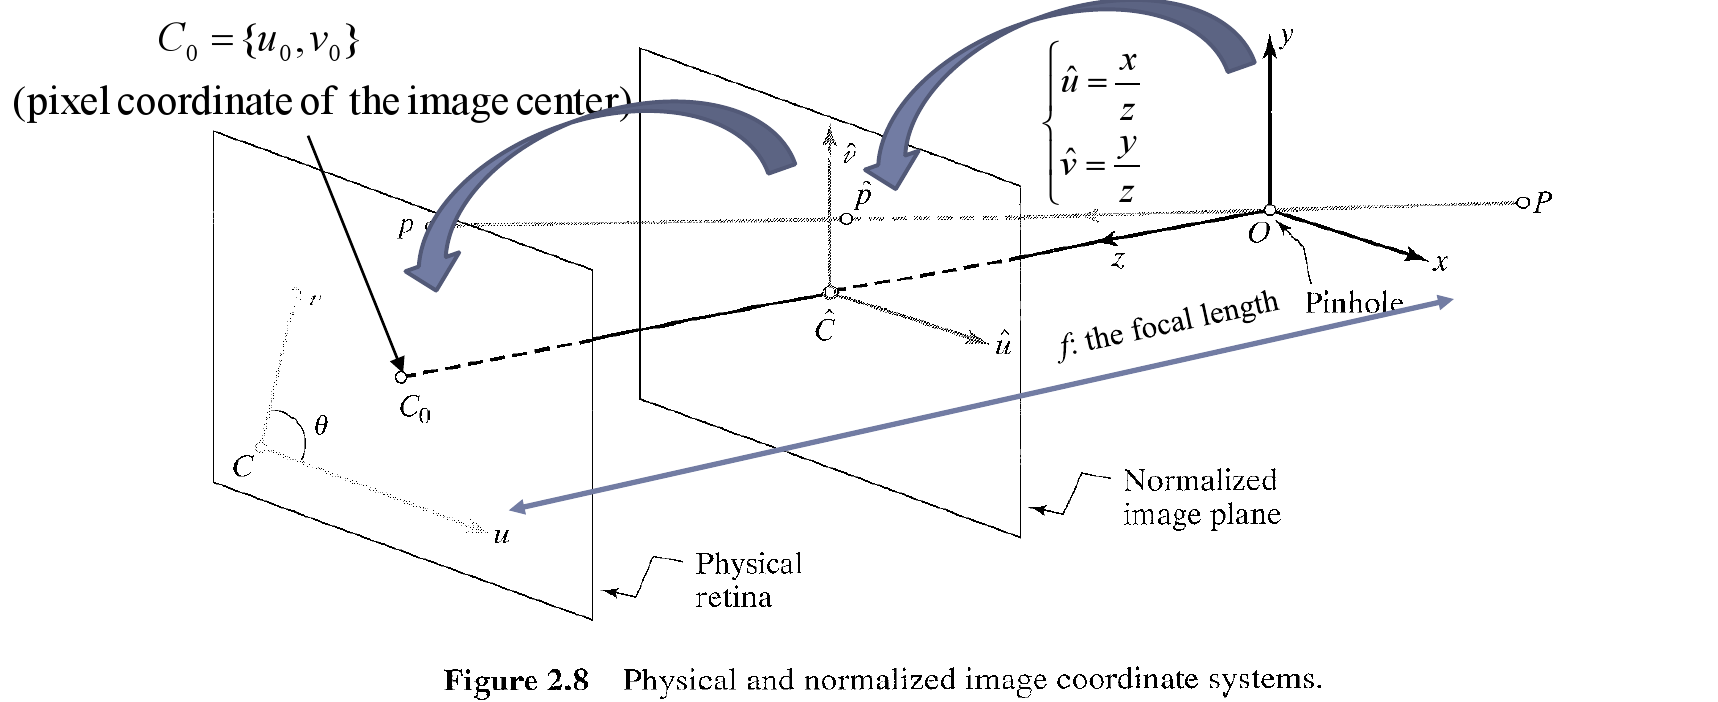
\includegraphics[width=.8\textwidth]{physic-normalized-img-coord.png}
\caption{Intrinsic parameters relates the physical image, $p$, to a normalized image plane $\hat{p}$ by solving equations for affine and perspective projection. Parameter $\alpha, \beta$ are the product of focal length and pixel resolution. $\theta$ is the angle between horizontal and vertical axis. $u_0, v_0$ are the center of the physical image. First pinhole coordinate in projected on $\hat{p}$ using perspective projection. $\hat{p}$ is projected on $p$ using affine projection.}
\end{figure}
\end{frame}

\begin{frame}
\begin{columns}[T] % align columns
\begin{column}{.5\textwidth}
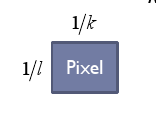
\includegraphics[width=.7\textwidth]{pixel_k_l.png}\vfill
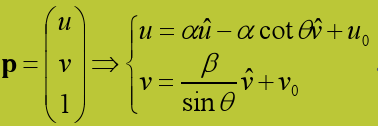
\includegraphics[width=\textwidth]{p.png}
\end{column}

\begin{column}{.5\textwidth}
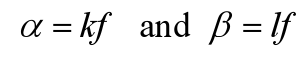
\includegraphics[width=\textwidth]{alpha_beta_def.png}\vfill
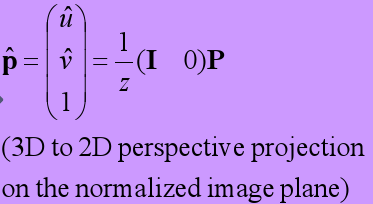
\includegraphics[width=\textwidth]{p_hat.png}
\end{column}
\end{columns}\vfill

\begin{columns}[T] % align columns
\begin{column}{\textwidth}
Converting the coordinates in homogeneous for makes these equation computationally suitable for optimization. All the intrinsic parameters can be encoded into a matrix K.
\end{column}
\end{columns}

\end{frame}


\begin{frame}
\frametitle{Intrinsic Parameters}
\begin{figure}
\centering
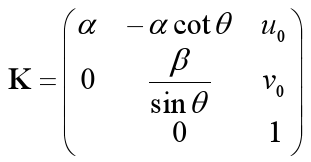
\includegraphics[width=.4\textwidth]{k_mat.png}\vfill
All the intrinsic parameters are encoded in the projection matrix K. ($\hat{p}$'s projection on p).\vfill
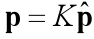
\includegraphics[width=.15\textwidth]{p_eq_kp_hat.png}\vfill
Can rewritten as,\vfill
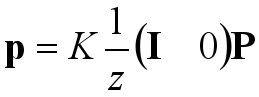
\includegraphics[width=.3\textwidth]{p_eq_K_1_2_I_0_P.png}\vfill
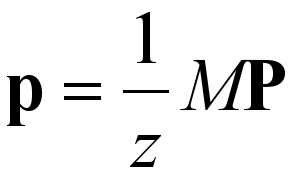
\includegraphics[width=.28\textwidth]{p_eq_MP.png}\vfill
\end{figure}
\end{frame}

\subsection{Extrinsic Parameters}
\begin{frame}
\begin{figure}
\centering
\frametitle{Extrinsic Parameters}
Real physical world coordinate W is not P. Extrinsic parameters are used to relate W to P.\vfill
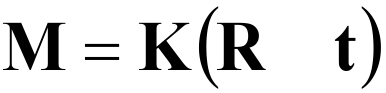
\includegraphics[width=.3\textwidth]{M_eq_KRT.png}\vfill
\end{figure}
\end{frame}

\subsection{Basic Theory}
\begin{frame}
\begin{figure}
\centering
\frametitle{Basic Theory of the Project}
z is not independent of M and P. Thus\vfill
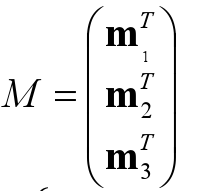
\includegraphics[width=.24\textwidth]{m123.png}\vfill
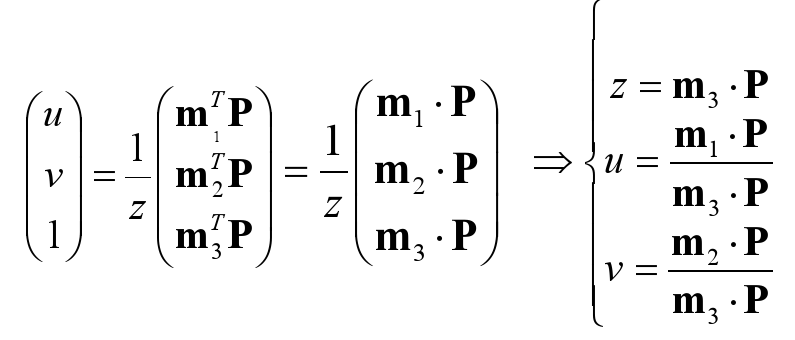
\includegraphics[width=.7\textwidth]{u_v.png}
\end{figure}
\end{frame}

\begin{frame}
\begin{figure}
\centering
\frametitle{Basic Theory of the Project}
For n given World coordinates the parameter can be solved using the following linear system\vfill
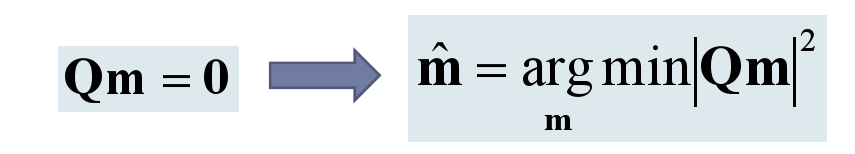
\includegraphics[width=.5\textwidth]{opt_M.png}\vfill
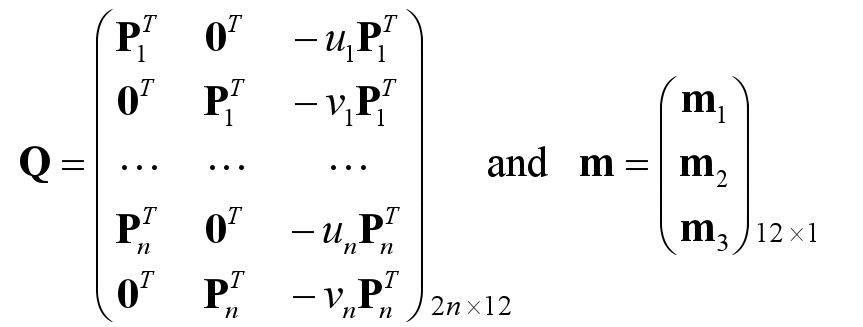
\includegraphics[width=.7\textwidth]{Q.png}\vfill
In the project the \say{model.dat} \& \say{observe.dat} file contained all information to build P and $u,v$ respectively to calculate Q. The first task was to estimate projection matrix $M$. Other tasks involved manipulating $M$ to calculate extrinsic and intrinsic parameters and 2D locations of given 3D locations. 
\end{figure}
\end{frame}

\subsection{Estimation of Parameters}
\begin{frame}
\frametitle{Estimation of Intrinsic and Extrinsic Parameters}
\begin{figure}
\centering
When projection matrix $M$ is calculated it can divided into blocks\vfill
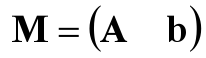
\includegraphics[width=.3\textwidth]{mab.png}\vfill
Using a scaling factor $\rho$ we can define 
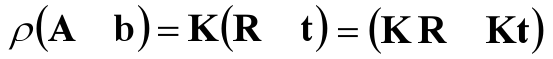
\includegraphics[width=.5\textwidth]{rab.png}
\end{figure}
\end{frame}

\begin{frame}
\frametitle{Estimation of Intrinsic Parameters}
\begin{figure}
\centering
Intrinsic parameters can be calculated using the constraint that $\rho a_3$ is always $\pm1$ because rows of a rotation matrix is has unit length\vfill
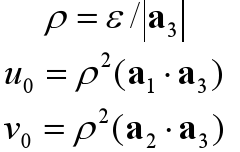
\includegraphics[width=.3\textwidth]{rouv.png}\vfill
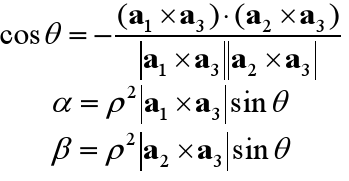
\includegraphics[width=.5\textwidth]{theta_alpha_beta.png}
\end{figure}
\end{frame}

\begin{frame}
\frametitle{Estimation of Extrinsic Parameters}
\begin{figure}
\centering
Extrinsic parameters can be calculated using\vfill
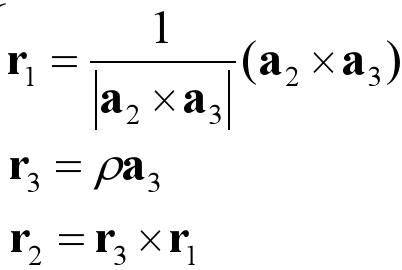
\includegraphics[width=.3\textwidth]{R.png}\vfill
Where the key term is to calculate $r_3$ having calculated $\rho$. The cross products follow that right hand rule.\vfill
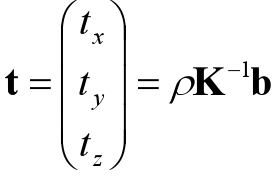
\includegraphics[width=.3\textwidth]{t.png}\vfill
\end{figure}
\end{frame}

\section{Result}
\subsection{Parameters}
\begin{frame}
\frametitle{Result}
\begin{columns}[T] % align columns
\begin{column}{.6\textwidth}
\begin{table}
	\resizebox{.9\linewidth}{!}{
	\pgfplotstabletypeset[%
	   column type=,
	   dec sep align,
	   fixed zerofill,
	   precision=3,
	   col sep=space,
	   columns/0/.style ={column name=},
	   columns/1/.style ={column name=},
	   columns/2/.style ={column name=},
	   columns/3/.style ={column name=},
	   every head row/.style={after row=\toprule},
	   every last row/.style={after row=\bottomrule},
	   ]{M.csv}
	}
	\caption{Projection Matrix M}
\end{table}\vfill
\end{column}

\begin{column}{.4\textwidth}
\begin{table}
	\resizebox{.9\linewidth}{!}{
	\pgfplotstabletypeset[%
	   column type=,
	   dec sep align,
	   fixed zerofill,
	   precision=3,
	   col sep=space,
	   columns/0/.style ={column name=},
	   columns/1/.style ={column name=},
	   columns/2/.style ={column name=},
	   columns/3/.style ={column name=},
	   every head row/.style={after row=\toprule},
	   every last row/.style={after row=\bottomrule},
	   ]{K.csv}
	}
	\caption{K}
\end{table}\vfill
\end{column}
\end{columns}
\end{frame}

\subsection{Extrinsic Parameter}
\begin{frame}
\frametitle{Extrinsic Parameter}
\begin{table}
	\resizebox{.8\linewidth}{!}{
	\pgfplotstabletypeset[%
	   column type=,
	   dec sep align,
	   fixed zerofill,
	   precision=3,
	   col sep=space,
	   columns/0/.style ={column name=},
	   columns/1/.style ={column name=},
	   columns/2/.style ={column name=},
	   columns/3/.style ={column name=},
	   every head row/.style={after row=\toprule},
	   every last row/.style={after row=\bottomrule},
	   ]{R.csv}
	}
	\caption{Rotation Matrix R}
\end{table}\vfill

\begin{table}
	\resizebox{!}{.2\textheight}{
	\pgfplotstabletypeset[%
	   column type=,
	   dec sep align,
	   fixed zerofill,
	   precision=3,
	   col sep=space,
	   columns/0/.style ={column name=},
	   columns/1/.style ={column name=},
	   columns/2/.style ={column name=},
	   columns/3/.style ={column name=},
	   every head row/.style={after row=\toprule},
	   every last row/.style={after row=\bottomrule},
	   ]{t.csv}
	}
	\caption{Translation Vector t}
\end{table}\vfill

\end{frame}

\subsection{Intrinsic Parameter}
\begin{frame}
\frametitle{Intrinsic Parameter}
\centering
$\theta=85.027358933^\circ$\\
$\alpha=41408.8860516$\\
$\beta=27810.7780862$\\
$u_0=20591.9094866$\\
$v_0=5116.87372168$\\
\end{frame}

\subsection{Visualization}
\begin{frame}
\frametitle{Result}
\begin{figure}
\centering
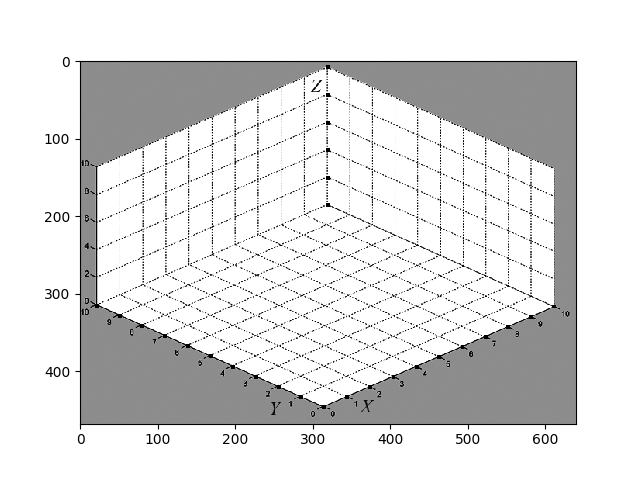
\includegraphics[height=.6\textheight]{Figure_1-1.png}\vfill
\caption{Plot of input data in model file using window size 4. The plot shows the input matches with the projection. It implies two things; the input data and the calculated projection matrix both are correct. The same window size has been used throughout the project. Here window size is the number of pixel which has been blacken out to draw a dot.}
\end{figure}
\end{frame}

\begin{frame}
\frametitle{Result}
\begin{figure}
\centering
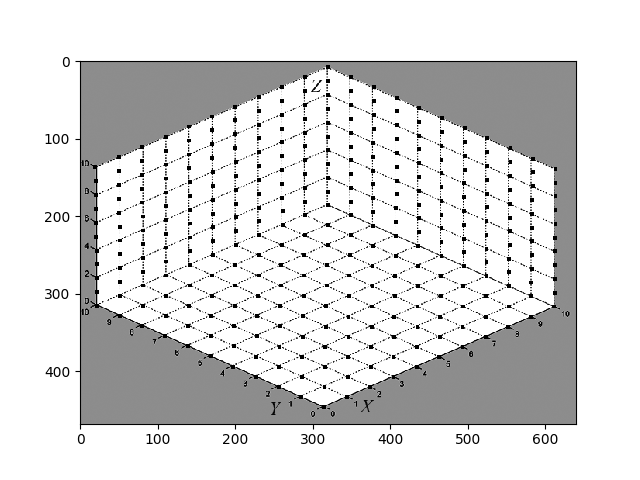
\includegraphics[height=.6\textheight]{Figure_1.png}\vfill
\caption{In the project generated 3D coordinate data and projected them on 2D image. The dots matches the coordinate.}
\end{figure}
\end{frame}

\begin{frame}
\frametitle{Result}
\begin{figure}
\centering
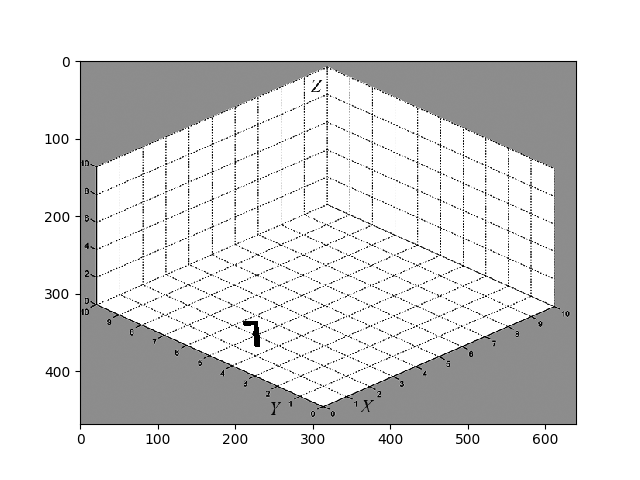
\includegraphics[height=.6\textheight]{tablelamp.png}\vfill
\caption{Table lamp projected from a public 3D data set\footnote{http://pointclouds.org/media/}.}
\end{figure}
\end{frame}

\begin{frame}
\frametitle{Result}
\begin{figure}
\centering
\movie[height=4cm, width=6cm, autostart,loop, poster, duration=5s]{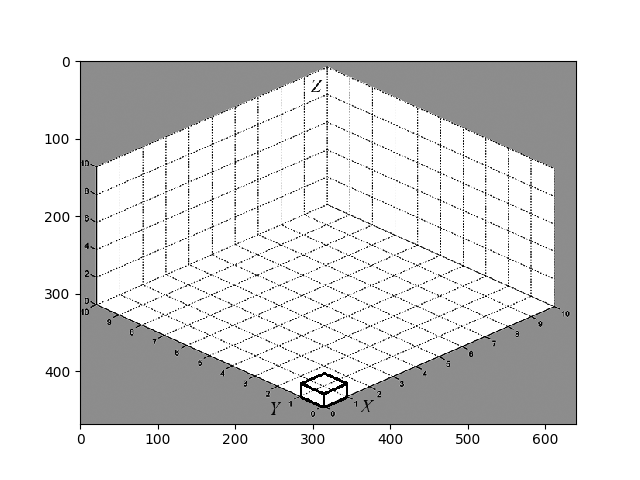
\includegraphics[height=4cm, width=6cm]{Figure_1-2.png}}{vdo.mp4}
\caption{A 3D box has been created using 7 vertices and 8 lines. 100 sample 3D points has been used to represent the line. The animation emulates the movement of the box by moving the points along X axis}
\footnote{N.B. The videos and the presentation pdf file should be in the same directory. phonon-backend-vlc or updated should be installed for Okular pdf reader. For adobe reader real time player plugin should be installed}
\end{figure}
\end{frame}

\begin{frame}
\frametitle{Result}
\begin{figure}
\centering
\movie[height=4cm, width=6cm, autostart,loop, poster, duration=5s]{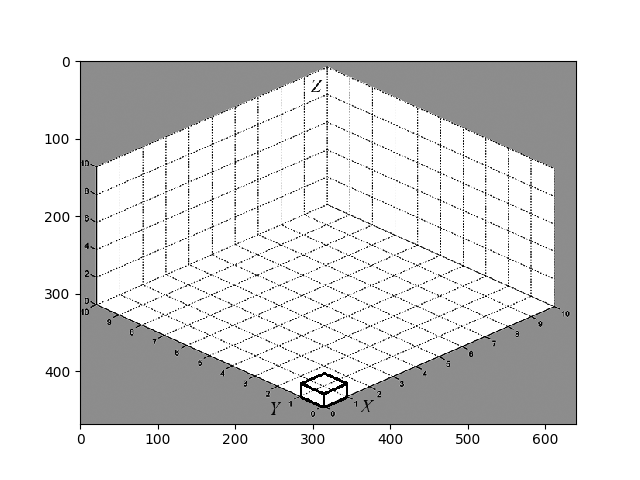
\includegraphics[height=4cm, width=6cm]{Figure_1-2.png}}{diag_move.mp4}
\caption{Similar to previous video but now it shows my implementation can move the box diagonally.}
\footnote{N.B. The videos and the presentation pdf file should be in the same directory. phonon-backend-vlc or updated should be installed for Okular pdf reader. For adobe reader real time player plugin should be installed}
\end{figure}
\end{frame}

\begin{frame}
\frametitle{Result}
\begin{figure}
\centering
\movie[height=4cm, width=6cm, autostart,loop, poster, duration=5s]{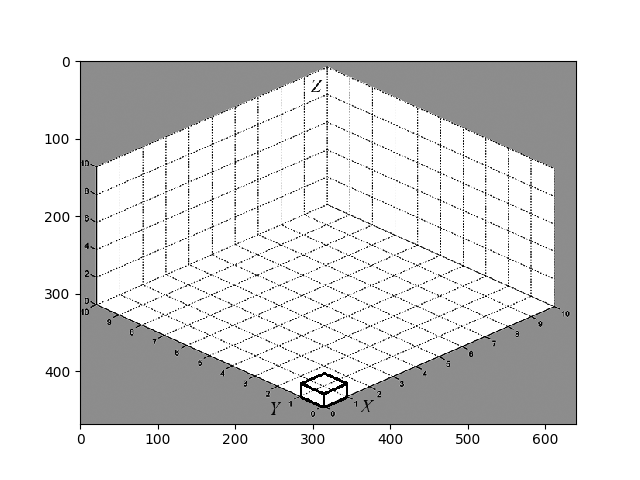
\includegraphics[height=4cm, width=6cm]{Figure_1-2.png}}{different_origin.mp4}
\caption{Similar to previous two videos but now it shows my implementation can have different original position and arbitrary goals in the space.}
\footnote{N.B. The videos and the presentation pdf file should be in the same directory. phonon-backend-vlc or updated should be installed for Okular pdf reader. For adobe reader real time player plugin should be installed}
\end{figure}
\end{frame}

\begin{frame}
\frametitle{Experiment With Different Parameter}
\begin{itemize}
	\item We were give 27 world coordinates and image pixel coordinate in input
	\item I have manually added $(5,10,0),(10,5,0)$ in model and corresponding pixel $(171,250), (465,251)$  in observation using Gimp Image editor and then run the program.
	\item I have found that adding more observation increases the accuracy of projection
	\item I have defined the accuracy as the difference between the projected 2D observation and actual observation $E = \dfrac{||A - B||}{N}$. Where N is the number of observation.
\end{itemize}
\begin{table}[]
\centering
\caption{Effect of Changing Parameters}
\label{my-label}
\begin{tabular}{|l|l|l|}
\hline
N  & E                    & theta (in deg) \\ \hline
27 & 0.097990 & 85.027358  \\ \hline
28 & 0.094491 & 85.033215  \\ \hline
29 & 0.091232 & 91.722549  \\ \hline
\end{tabular}
\end{table}

This result suggest that more observation data as input will create better projection. The change in $\theta$ also suggests that for better accuracy we may increase $\theta$ somehow. One possibility is changing the viewing angle. 
\end{frame}

\section{Conclusion}
\begin{frame}
\frametitle{Conclusion}
\begin{itemize}
	\item In this project, we have studied the linear method for geometric camera calibration
	\item We have implemented in Python
	\item We have verified our result by projecting and visualizing 3D points from the world coordinate to 2D image plane.
\end{itemize}
\end{frame}

% ------------------------------------------------------------------------------------------------------------------

\section{Conclusion}
\begin{frame}
\frametitle{Conclusion}
\begin{columns}
\column{\textwidth}
\centering
\begin{itemize}
\item \textbf{Thank You}
\item \textbf{Questions ?}
\end{itemize}
\end{columns}
\end{frame}

% ------------------------------------------------------------------------------------------------------------------

\end{document}

